\documentclass[10pt,a4paper,oneside]{scrartcl}

% packages
\usepackage{scrhack}
\usepackage{fullpage}
\usepackage{graphicx}
\usepackage[style=numeric,backend=bibtex8,urldate=iso8601]{biblatex}
\usepackage{listings}
\usepackage{courier}
\usepackage{array}
\usepackage{tabularx}
\usepackage{amsmath}
\usepackage{longtable}
\usepackage[iso]{datetime}
\usepackage{pdfpages}
\usepackage[utf8]{inputenc}

% basic latex configuration
\setlength{\parskip}{\baselineskip}
\setlength{\parindent}{0pt}

% biblatex
\addbibresource{references.bib}

% graphics
\graphicspath{ {./images/} }

% language listings
\lstdefinelanguage{CL}[ANSI]{C}
{
	morekeywords={__kernel,kernel,__local,local,__global,global,__constant,constant,__private,private},
	morekeywords={char2,char3,char4,char8,char16,uchar,uchar2,uchar3,uchar4,uchar8,uchar16,short2,short3,short4,short8,short16,ushort,ushort2,ushort3,ushort4,ushort8,ushort16,int2,int3,int4,int8,int16,uint,uint2,uint3,uint4,uint8,uint16,long2,long3,long4,long8,long16,ulong,ulong2,ulong3,ulong4,ulong8,ulong16,float2,float3,float4,float8,float16,image2d_t,image3d_t,sampler_t,event_t,bool,bool2,bool3,bool4,bool8,bool16,half2,half3,half4,half8,half16,quad,quad2,quad3,quad4,quad8,quad16,complex,imaginary},
	morekeywords={convert_char2,convert_char4,convert_char8,convert_char16,convert_uchar,convert_uchar2,convert_uchar4,convert_uchar8,convert_uchar16,convert_short,convert_short2,convert_short4,convert_short8,convert_short16,convert_ushort,convert_ushort2,convert_ushort4,convert_ushort8,convert_ushort16,convert_int,convert_int2,convert_int4,convert_int8,convert_int16,convert_uint,convert_uint2,convert_uint4,convert_uint8,convert_uint16,convert_long,convert_long2,convert_long4,convert_long8,convert_long16,convert_ulong,convert_ulong2,convert_ulong4,convert_ulong8,convert_ulong16,convert_float,convert_float2,convert_float4,convert_float8,convert_float16}
	morekeywords={write_imagef,write_imagei,write_imageui,read_imagef,read_imagei,read_imageh,read_imageui,get_image_width,get_image_height,get_image_depth,get_image_channel_data_type,get_image_channel_order,get_image_dim,get_work_dim,get_global_size,get_global_id,get_local_size,get_local_id,get_num_groups,get_group_id,cross,dot,distance,length,normalize,fast_distance,fast_normalize,isequal,isnotequal,isgreater,isgreat,erequal,isless,islessequal,islessgreater,isfinite,isinf,isnan,isnormal,isordered,isunordered,signbit,any,bitselect,select,async_work_group_copy,wait_group_events,prefetch,barrier,mem_fence,read_mem_fence,write_mem_fence,acos,acosh,acospi,asin,asinh,asinpi,atan,atan2,atanh,atanpi,atan2pi,cbrt,ceil,copysign,cos,cosh,cospi,erfc,erf,exp,exp2,exp10,expm1,fabs,fdim,floor,fma,fmax,fmin,fmod,fract,floor,frexp,hypot,ilogb,ldexp,lgamma,lgamma_r,log,log2,log10,log1p,logb,mad,modf,nan,nextafter,pow,pown,powr,remainder,remquo,rint,rootn,round,rsqrt,sin,sincos,sinh,sinpi,sqrt,tan,tanh,tanpi,tgamma,trunc,half_cos,half_divide,half_exp,half_exp2,half_exp10,half_log,half_log2,half_log10,half_powr,half_recip,half_rsqrt,half_sin,half_sqrt,half_tan,native_cos,native_divide,native_exp,native_exp2,native_exp10,native_log,native_log2,native_log10,native_powr,native_recip,native_rsqrt,native_sin,native_sqrt,native_tan,mad24,mul24,mul_hi,sub_sat,rotate,mad_sat,clz,rhadd,hadd,add_sat,abs_diff,abs,max,min,upsample,get_global_offset,minmag,maxmag,clamp,async_work_group_strided_copy,vec_step,shuffle,shuffle2}
	sensitive=true,
	morecomment=[l]{//},
	morecomment=[s]{/*}{*/},
	morestring=[b]",
}

\lstset
{
	tabsize=2,
	captionpos=b,
	basicstyle=\ttfamily{},
	aboveskip=\parskip,
% keywordstyle=\color{blue}\bfseries,
% commentstyle=\color{commentgreen},
% stringstyle=\color{red},
	showstringspaces=false,
	breaklines=true,
	numbers=left,
	frame=single,
% backgroundcolor=\color{lightgray}
}

\title{GPGPU accelerated visualization of complex geometries}
%\subtitle{}
\author{Bernhard Manfred Gruber}
\date{\today}

\begin{document}


\includepdf{titlepage}
%\maketitle
%\thispagestyle{empty}
%\clearpage

\pagenumbering{Roman}

\section*{Declaration}

I hereby declare and confirm that this thesis is entirely the result of my own original work. Where other sources of information have been used, they have been indicated as such and properly acknowledged. I further declare that this or similar work has not been submitted for credit elsewhere.

\vspace{2cm}

\parbox{7cm}{
	\centering
	\rule{6cm}{1pt}\\
	Hagenberg, \today 
}
\hfill
\parbox{7cm}{
	\centering
	\rule{6cm}{1pt}\\
	Bernhard Manfred Gruber
}

%\section*{Acknowledgments}

Herwig Mayr for helping me to get the internship.

Alexander Leutgeb for excellent support.

RISC Software GmbH for providing me with an awesome work station.

Michael Hava for deepening my knowledge about C++11.

\section*{Kurzfassung}

Diese Arbeit stellt eine detaillierte Dokumentation über das Berufspraktikum des Autors bei der RISC Software GmbH dar. Nach einer kurzen Einführung in das Unternehmen sowie das Projekt Enlight werden die Ziele des Praktikums erläutert, welche verschiedene Aspekte der Implementierung eines Raycasters mit OpenCL betreffen, der in den drei Praktikumsmonaten erstellt wurde.

Im Anschluss an die Einführung werden grundlegende Themen sowie Basiswissen behandelt, das in späteren Kapiteln benötigt wird. Dazu gehört ein Grundverständnis über Raycasting, reguläre Gitter als Beschleunigungsstruktur, Raycasting implizit beschriebener Geometrie über boolsche Subtraktion und OpenCL als Technologie für GPU Beschleunigung.

Bevor sich die Arbeit in die eigentliche Implementierung vertieft, wird der zum Praktikumsbeginn bestehende Prototyp detailliert analysiert. Dabei wird vor allem auf fortgeschrittene Algorithmen zur Optimierung des eingesetzten Raycasting Verfahrens eingegangen.

Anschließend fokussiert sich die Arbeit auf verschiedenen OpenCL Programme, deren Ziel es ist GPU beschleunigt Bilder in ähnlicher Qualität wie die existierende Implementierung zu erzeugen. Auf Vorteile und Schwierigkeiten während der Implementierung der OpenCL Programme wird ebenfalls eingegangen.

Die abschließenden Laufzeitvergleiche der funktionierenden OpenCL Raycaster mit der existierenden CPU Implementierung werden noch durch Erfahrungen mit Entwicklungswerkzeugen rund um OpenCL und einer kurzen Diskussion über noch offene Probleme abgerundet.

\pagebreak

\section*{Abstract}

This thesis provides a detailed coverage of the authors internship at RISC Software GmbH. After a short introduction to the company and the Enlight project, the goals of the internship are discussed, which address various aspects of an OpenCL ray caster implementation created during the three months working period.

In succession to the introduction, fundamental topics required in further chapters of the thesis are covered. These include the principle of ray casting, regular grids as acceleration structure, ray casting implicitly described geometry using boolean subtraction and OpenCL as technology for GPU acceleration.

Before the thesis deepens into the actual implementation, the existing prototype at the start of the internship is analyzed in detail. This includes advanced algorithms to optimize the used ray casting approach.

The primary focus then lies on several OpenCL programs with the goal of reproducing the visual output of the existing CPU implementation using GPU acceleration. Advantages and difficulties of developing with OpenCL are encountered during the explanations of the implementations.

The final benchmarks of the working OpenCL ray casters are than rounded off by experiences made with various development tools around OpenCL and a discussion of the still remaining problems.


\tableofcontents

\clearpage

\pagenumbering{arabic}

\section{Introduction}

\subsection{Motivation}

For a long time the speed of algorithms experienced a constant growth through improved processor hardware. Intel co-founder Gordon E. Moore was one of the first persons to describe this trend in 1965. This description is well known by the name Moore's law which initially stated that the number of transistors on an integrated circuit doubles every year \cite{moore_law}. This trend slowed down and Moore had to change the interval to two years a decade later \cite{moore_law_2003}. The most important consequence however has been realized by one of Moore's co-workers at Intel, David House, who predicted that the performance of processors would double every 18 months \cite{moore_law_2003}. As a result, an increase in computing power could be obtained simply by running the same algorithms on newer hardware. As a consequence, hardware dominated the growth of algorithms' performance for a long period of time.

Unfortunately, processing hardware technologies hit a limit at the beginning of the third millennium. Physical bounds, like the size of atoms, prevented a further shrink of integrated circuits which would allow an increase in clock speed. Therefore, processor vendors like Intel and AMD started to place multiple CPUs on a single chip which still lead to an increase in computational power but in a different way than in the last 40 years. This change is sometimes referred to as the multicore crisis \cite{multicore_crisis}. The consequence from a software developer's perspective is that traditional algorithms stopped gaining speed by being run on newer hardware. In fact, improving performance is now up to the programmer, who is responsible for writing concurrent and parallel software that can make full use of the underlying hardware's capabilities. 

But multicores were not the only major hardware change that had an impact on the way software is developed recently. Graphics cards, which were initially intended to offload and accelerate 2d and 3d graphic operations from the CPU to a separate hardware device, started to gain popularity in non graphical areas of programming. A GPUs intense float processing power and parallel nature by design makes it ideal for uses in several areas of science, business and engineering (General Purpose GPU). When used in the right place, a GPU may compute results several magnitudes faster than the CPU \cite{gpu_history}. However, due to the very different hardware architecture the graphics card is still not suitable to efficiently solve the same problems as a CPU does.

Todays software engineers working in performance focused domains have a hard time designing their applications and algorithms. With two very different types of processors (CPU and GPU), both excellent in their own ways, and a lot of APIs and frameworks around them (OpenMP, CUDA, OpenCL, DirectCompute, C++ AMP, ...), the available hardware and software to access it is more heterogeneous than ever. Thus, profound knowledge of the available technologies, their performance and restrictions as well as the consequences for a development team is essential for choosing the optimal strategy to tackle todays computational needs.

\subsection{Goal}
The goal of this thesis is to provide the reader with a state of the art comparison of modern GPU and CPU performance in solving traditional problems such as sorting arrays and multiplying matrices using various approaches.
The GPU algorithms will be implemented using the Open Computing Language (OpenCL). Therefore the reader is given a short introduction into OpenCL in order to understand the provided code samples and how programming for a GPU works. These OpenCL implementations are benchmarked against algorithms implemented in C/C++ solving the same problem. It is important to note that the GPU and CPU version do not necessarily have to use the same algorithm, they only have to output the same result. This decision was inevitable due to the highly diverse hardware properties of the CPU and the GPU.
The problems chosen for this comparison are sorting an array, multiplying two large matrices and calculating the parallel prefix sum of an array (explained in corresponding chapter \ref{sec:prefix_sum}). These algorithms cover several different aspects that play an important role when implementing an algorithm for a GPU such as runtime complexity, memory footprint and memory transfer time vs. computation time. 

Eventually, the results of benchmarking the chosen algorithms should give the reader an idea how much a GPU can accelerate different kinds of algorithms and what a programmer has to pay attention to when developing GPGPU accelerated software. This knowledge is not only valuable during developing but also useful when choosing the right technology for a given problem. This thesis should aid all software engineers in understanding how GPU computing works and where it should be used.

\subsection{History of GPGPU Computing} 
\label{sec:history}
Before we start into details about OpenCL and several GPU implementations, some background information about how GPUs have evolved is provided which may help understanding the design and peculiarities of graphics hardware. The following information is taken from a paper survey in 2010 \cite{gpu_history}.

In the early 1980's a "GPU" was nothing more than an integrated frame buffer, an additional chip that relied on the CPU for drawing.

One of the first dedicated video cards was the IBM Professional Graphics Controller (PGA) released in 1984. It used an on-board Intel 8088 microprocessor to take care of graphical calculations in order to take off load from the main processor. Although the Intel 8088 was in fact a conventional CPU, the PGA's separate on-board processing unit marked an important step towards the development of GPUs as co-processors.

In the following years more graphics orientated features where added like shading, lighting, rasterization, the depth buffer and color blending. With the introduction of OpenGL in 1989 by Silicon Graphics Inc. (SGI), the world's first application programming interface (API) for 2D and 3D graphics was released. OpenGL was designed upon a concept called the graphics pipeline which depicts video processing as data traveling through multiple stages of operations. The pipeline begins at the CPU by sending geometry data together with colors, textures etc., which is then transformed from the initial 3D coordinate space to pixel coordinates. Lighting operations use material colors and textures to shade the incoming triangles which are then rasterized into the frame buffer for display. As the programmer was not able to alter the functionality if the pipeline it is also well known under the term "fixed function pipeline". This processing model determined the design of graphics hardware for more then a decade.

In the mid 1990's NVIDIA, ATI and Matrox started to provide graphic controllers for consumers. Famous computer games like Quake and Doom became popular spurring the gaming industry and the interest in GPUs. However, GPUs at this time were only able to output one pixel per clock cycle and CPUs were able to send more triangles than the GPU could handle. This problem lead graphic hardware vendors to adding more pipelines and eventually more cores to their GPUs in order to enable parallel pixel processing and increase the throughput.

NVIDIA's release of the GeForce 3 in 2001 marked an important step in the evolution of GPUs by loosening the restrictions of the fixed function pipeline. With the ability of writing small programs for the GPU, which could operate on the vertices traveling through the pipeline, programmers were given a tool to make limited changes to the behavior of the pipeline. These programs were called vertex shaders and were written in an assembly-like language. One year later the pixel shader followed running on a separate part of the GPU hardware.

\begin{figure} % from http://wiki.ega.org.pl/images/b/b4/Pipeline.png
\centering
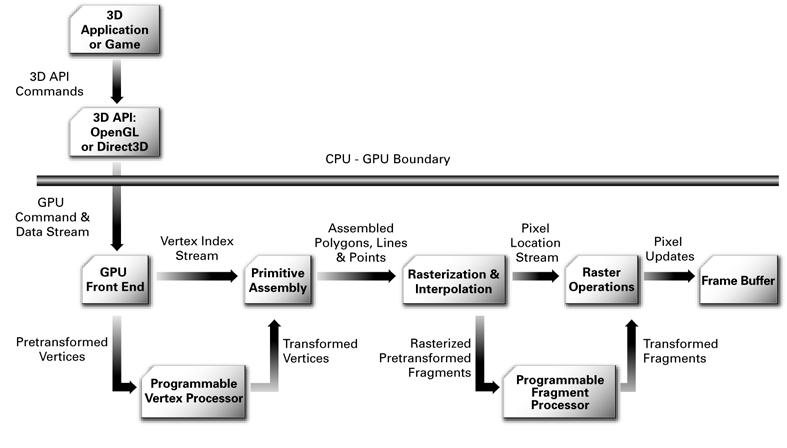
\includegraphics[width=0.7\linewidth]{pipeline2}
\caption{The graphics pipeline with programmable vertex and fragment processor. \cite{cg_book}}
\label{fig:pipeline2}
\end{figure}

With the introduction of the High Level Shading Language (HLSL) with DirectX 9 in 2003 programming GPU hardware became easier than with the previous shaders written in assembler. The first developers started to use the available programmability for non-graphical tasks. The first attempts of GPU computing emerged. A year later in 2004 Brook and Sh appeared representing the first languages targeting GPGPU computing.
Although the workflow of the GPU is still based on a programmable graphics pipeline, the hardware mainly consists of strong, highly parallel floating-point processors with fast memory access.

In 2006 the GeForce 8800 featured the first GPU with a unified programmable processor called a streaming multiprocessor which is used to execute the vertex, pixel and a new geometry shader. The graphics pipeline has become only a software concept used by graphic APIs such as OpenGL and DirectX.

Software GPGPU support was introduced by NVIDIA with the Compute Unified Device Architecture (CUDA). It offers a C like language to create general purpose programs (called kernels) that can be executed on the GPU. ATI followed with the ATI Stream technology and Microsoft introduced compute shaders with DirectX 10.

In 2010 NVIDIA released the first GPU based on their Fermi architecture which was explicitly designed for GPGPU computing. The GTX580 Fermi GPU released later that year contained 16 streaming multiprocessors with 512 CUDA cores and accessed 1.5 GiB GDDR5 RAM with a bandwidth of 192.4 GB/s \cite{gtx580_spec}.

\subsection{Chapter overview}

After this short introduction chapter \ref{sec:opencl} will continue with a comprehensive coverage of OpenCL. Beside general information about the API, this chapter focuses on the knowledge required to understand how OpenCL executes kernels on the GPU and what a developer has to pay attention to when programming for graphics hardware. This information is vital for understanding the implemented algorithms in the subsequent chapters.

Chapter \ref{sec:matrix_mul} will present the first OpenCL implementation of a standard algorithm by tackling multiplications of large floating point matrices. Beside a simply and naive approach, several possibilities of optimizations are discussed introducing graphic hardware features like shared memory, texture memory and vector types.

\pagebreak

Chapter \ref{sec:prefix_sum} continues with implementations of a prefix sum algorithm (also known as scan) - a ridiculous simple problem for a CPU due to its sequential nature. However, the linearity if the algorithm does not fit the architecture of a GPU. A tree based approach is discussed which is commonly used to partly parallelize linear algorithms.

Chapter \ref{sec:sorting} focuses sorting as one of the most famous problems in computer science. Several well performing CPU implementations such as C's qsort and C++'s std::sort will be compared with GPU sorting techniques using less popular algorithms such as the bitonic sorting network and radix sort.


\section{Fundamentals}

\subsection{Raycasting}

vs. raytracing
vs. conventional rendering

principle

image with camera and image plane

advantages/disadvantages of rendering with ray casting

\subsubsection{Acceleration structures}

why do we need acceleration structures?

kd trees
bounding volume hierarchy
BSP

regular grid

traversing

\subsubsection{Packet casting}

different traversing

frustum culling
cache coherence (of adjacent rays)
SIMD


\subsection{Boolean raycasting}

works equal to CSG (Constructive Solid Geometry), except resulting mesh is never explicitly generated

water-tight

\subsection{OpenCL}

GPU hw architecture, how do kernels work? NDRange, buffers


\section{Existing prototype}
\label{sec:existing_prototype}

At the beginning of the internship the existing code base, shortly described in Chapter \ref{sec:goals}, was analyzed in order to understand how the ray casting application has been organized and implemented. The application is written in C++ using Microsoft Visual Studio 2010 and 2012 in 64 bit mode. Besides the provided compilers from Microsoft, also Intel's C++ compiler is used during development to benefit from stronger optimization. The code heavily uses C++11 features and AVX SIMD instructions, thus limiting the application to rather up-to-date compilers supporting C++11 and newer hardware. AVX is supported since Intel's Sandy Bridge and AMD's Bulldozer series. Furthermore, OpenMP is used as a technology for high level parallelization, OpenGL for visualization and the Microsoft Foundation Class (MFC), a C++ wrapper of the Win32 API, for window management and user interaction.
Considering the implemented algorithms, single ray casting of scenes composed of subtraction volumes as shown in chapter \ref{sec:boolean_raycasting} using the 3D DDA algorithm discussed in Chapter \ref{sec:regular_grids} has been used in the beginning. However, the initial approach has later been replaced by a highly optimized and parallel packet ray caster using the slice traversing algorithm presented in Chapter \ref{sec:packet_casting}. The single ray variant can still be found in the code but is not used anymore.

\begin{figure}
\centering
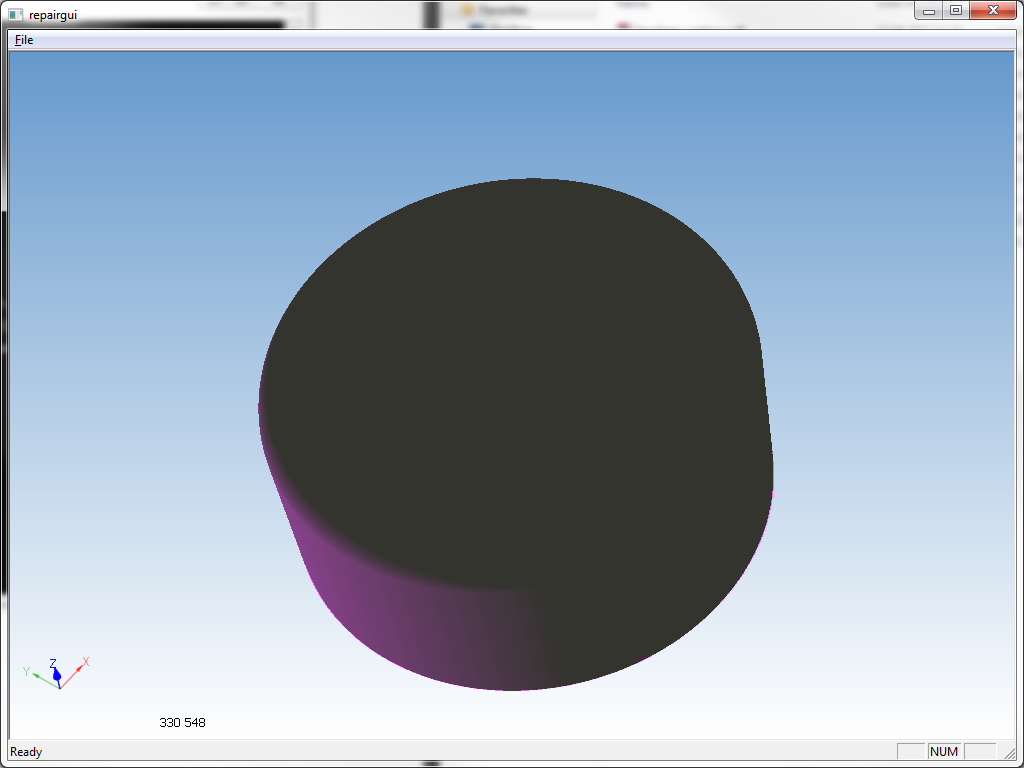
\includegraphics[width=0.49\textwidth]{cylinder_head_stock_gl}
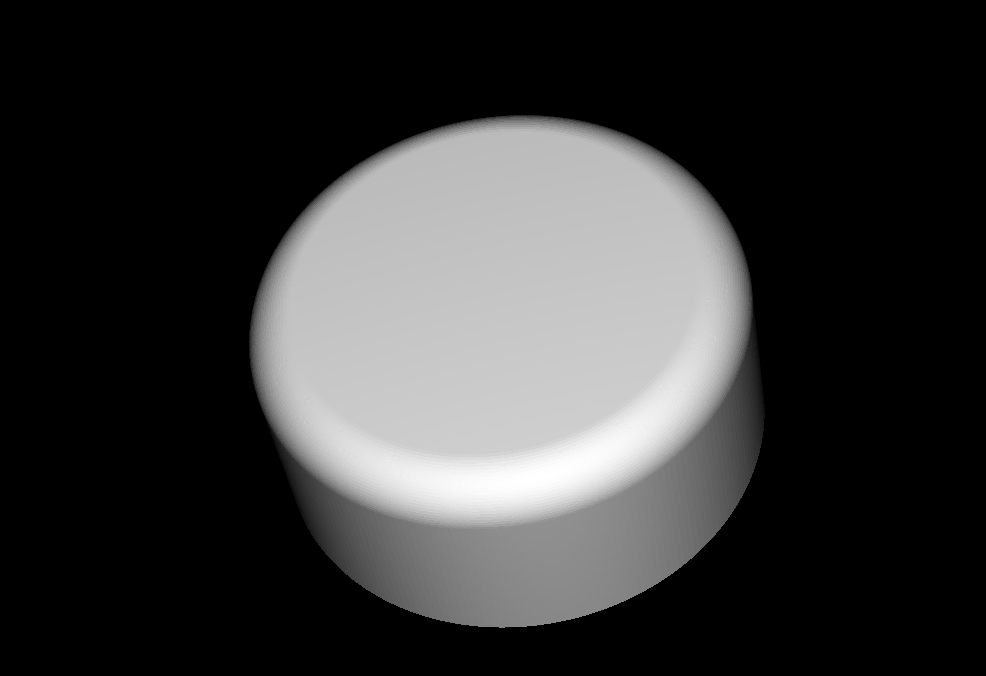
\includegraphics[width=0.49\textwidth]{cylinder_head_stock_cast_cpu}
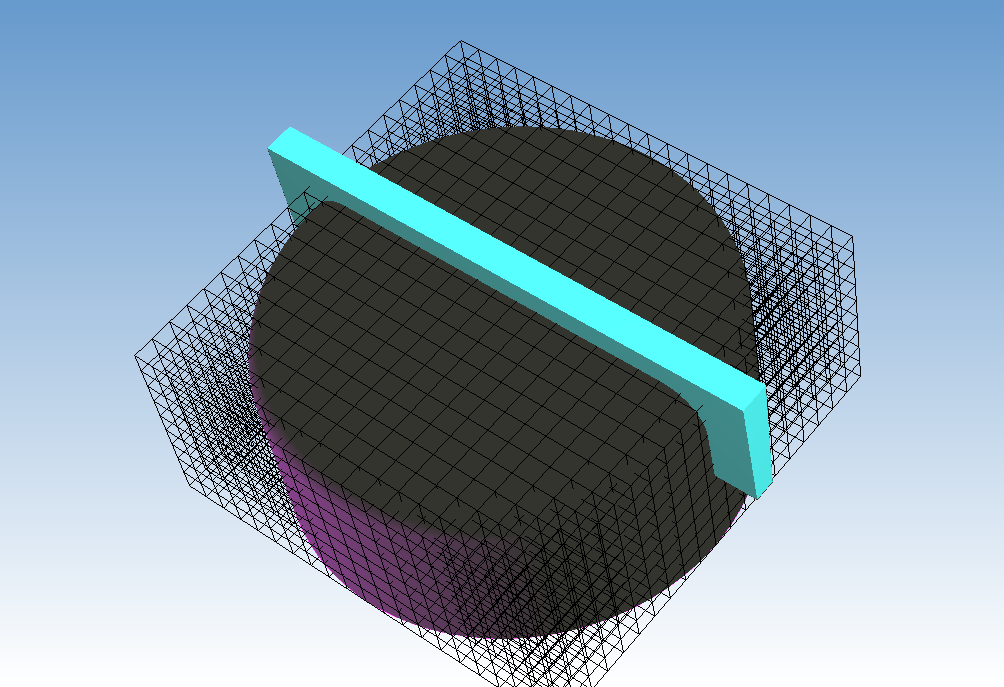
\includegraphics[width=0.49\textwidth]{cylinder_head_sub_gl}
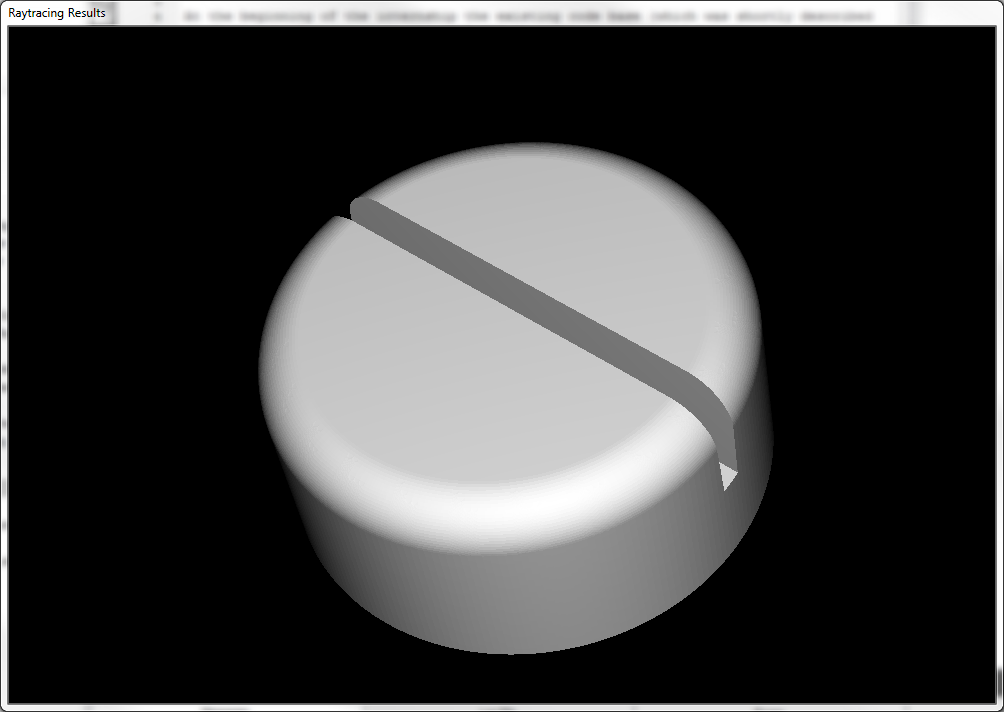
\includegraphics[width=0.49\textwidth]{cylinder_head_sub_cast_cpu}
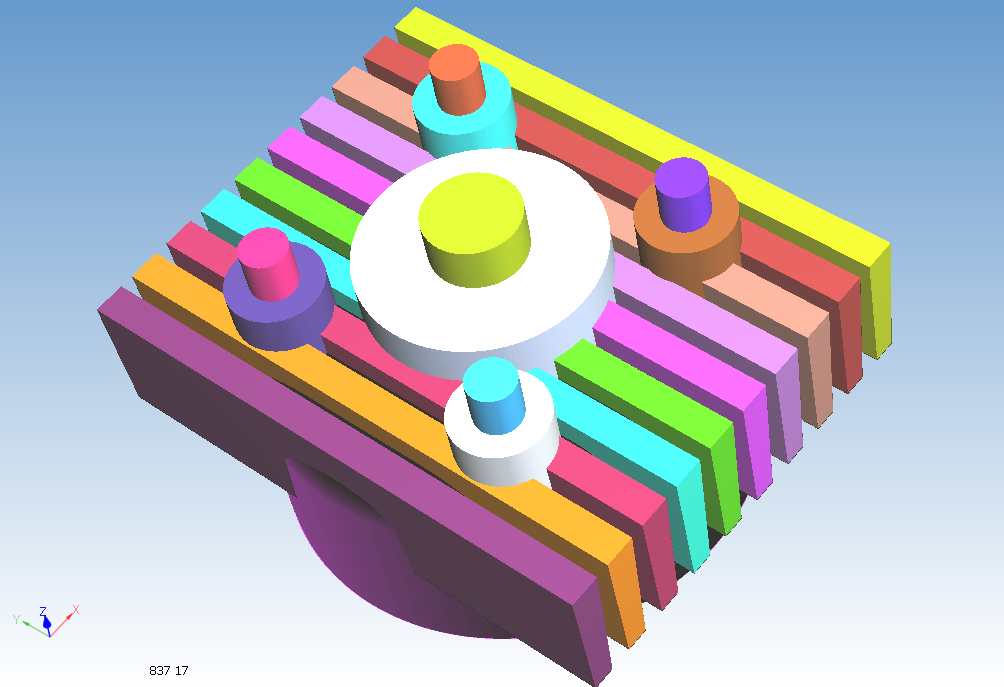
\includegraphics[width=0.49\textwidth]{cylinder_head_gl}
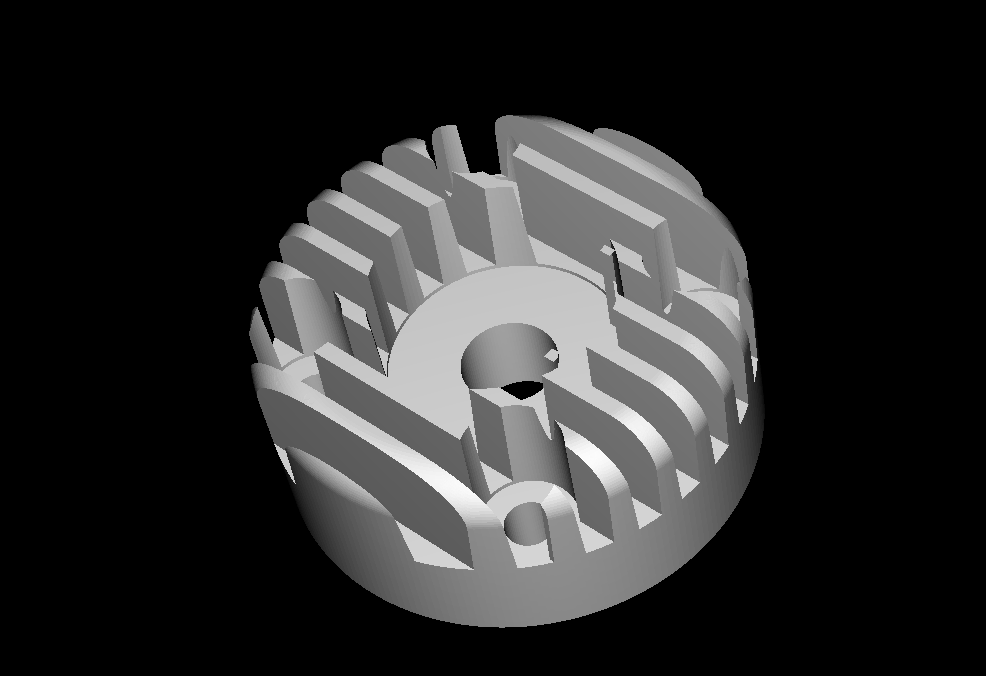
\includegraphics[width=0.49\textwidth]{cylinder_head_cast_cpu}
\caption{Screenshots of the existing prototype. The images on the left show the OpenGL visualizations of the loaded meshes. The images on the right show the ray casting result using the existing CPU packet ray caster. The first row only shows the loaded stock volume. The second row shows the stock volume and one subtraction volume. The OpenGL visualization also shows the grid. Note that the grid only has to cover the stock volume. The third row shows several subtraction volumes cut out of the stock forming a cylinder head.}
\label{fig:cylinder_head}
\end{figure}

\subsection{Structure}

Figure \ref{fig:enlight_class_diagram} shows a simplified class diagram of the most important classes used in the existing ray casting implementation. Most of them have been dealt with when extending the existing infrastructure by the new OpenCL ray caster.

\begin{figure}
\centering
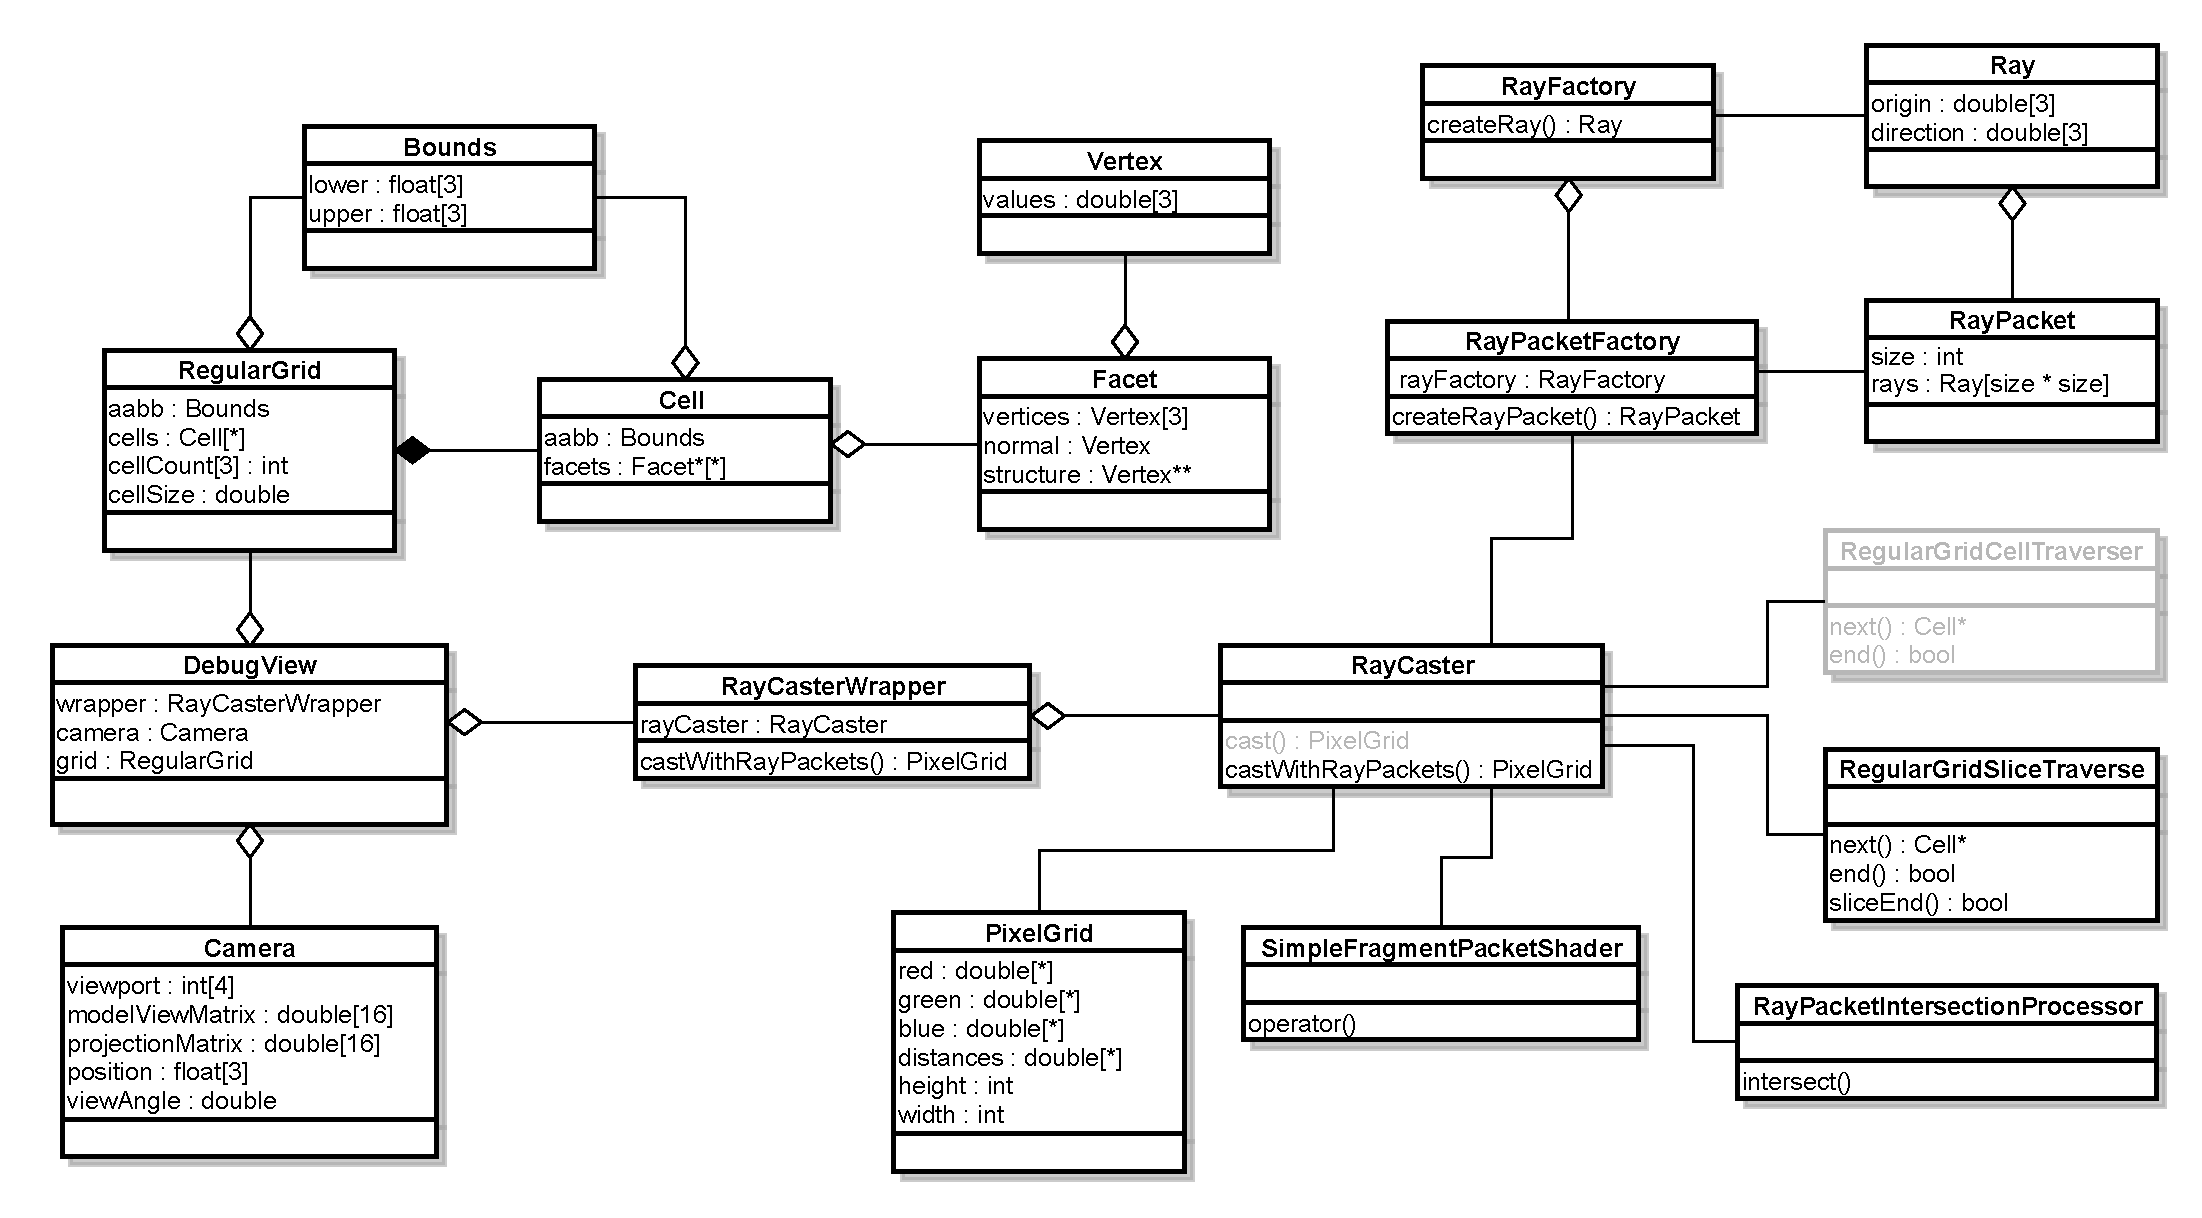
\includegraphics[width=\textwidth]{enlight_class_diagram}
\caption{Simplified class diagram of the most important classes involved in ray casting at the beginning of the internship.}
\label{fig:enlight_class_diagram}
\end{figure}

The central class containing most of the application logic is \lstinline!DebugView!. It inherits \lstinline!CWnd! from the MFC and is the main window of the application containing the OpenGL visualization. Besides all graphical user interactions, like zooming and rotating, using the cursor, also the console commands are parsed and processed by this class. It further contains an instance of \lstinline!Camera! which is updated according to user interaction. Also the regular grid holding all loaded meshes is stored by \lstinline!DebugView!. Finally, a ray caster wrapper class is also available (\lstinline!RayCasterWrapper!), which delegates calls to the actual ray casting implementation. When the application has been started, meshes can be loaded from the file system via corresponding console commands. The loaded meshes are processed by the classification algorithm and merged into the grid, cf. Chapter \ref{sec:classification}. Ray casting can be triggered either by issuing a command on the console or changing a camera property via GUI input (zoom, rotation). In both cases, \lstinline!DebugView! eventually invokes \lstinline!castWithRayPackets()! from the ray casting implementation wrapper and passes a reference to the grid and current camera settings. The wrapper delegates this call to the corresponding method in \lstinline!RayCaster! where the actual ray casting code is executed. Initially, several camera values are retrieved and a \lstinline!RayPacketFactory! is created. This factory relies on the older \lstinline!RayFactory! used for the initial single ray casting algorithm. Furthermore, an instance of \lstinline!PixelGrid! is created which will be later used to store the ray casting results and will be returned to the calling \lstinline!DebugView! class, where it is used to render the casted image. After this setup, the requested output image area, sized according to the width and height of the camera, is divided into a grid of square packets and iterated over by two nested for loops. The square size is adjustable and currently set to eight. The outer loop iterates over the rows of the packets and is executed in parallel using an OpenMP directive. Within the inner loop, \lstinline!RayPacket!s are created using the corresponding factory. Each packet is traversed through the grid using an instance of \lstinline!RegularGridSliceTraverser!. After the slice traverser has been initialized with the packet, which determines traversal axis and grid entry point, a while loop retrieves cells from the slice traverser using its \lstinline!next! method until \lstinline!end! returns true. On every slice end, the traversal may be early aborted if all rays of the packet have already hit. For each cell the slice traverser returns, the ray packet has to be intersected with the referenced triangles of this cell. This is done using an instance of \lstinline!RayPacketIntersectionProcessor!. This process consumes most of the required CPU time. Therefore the \lstinline!intersect! routine and all subroutines are highly optimized and highly consist of AVX vector intrinsics. The intersection test for the packet is performed in parallel using SIMD after all triangles of the cell have been culled against the frustum defined by the corner rays of the packet. Details are discussed later in Chapter \ref{sec:adapted_ray_casting}. For each intersection, the normal vector of the hit surface and the distance from the eye point are retrieved. The normal vector together with the initial ray direction of every ray of the packet is used by the \lstinline!SimpleFragmentPacketShader! to calculate a color value for the ray. Currently, the scalar product of both vectors is used to measure a gray scale value, achieve simple shading. The distance of the intersection point to the eye point (camera position), from which the ray originated, is later translated into the normal distance of the intersection point to the image plane which corresponds to the depth value which would have been generated by OpenGL if the scene has been rendered traditionally. After all ray packets have been processed, the final \lstinline!PixelGrid! instance containing the color and depth values is returned back to \lstinline!DebugView! for display.

\subsection{Ray casting data structure}
\label{sec:data_structure}

The data structure maintaining the geometry and accelerating the ray casting algorithm is implemented by several classes. To start with, the \lstinline!RegularGrid! class is a simple container for cells. It also stores some meta information such as the grids bounding box, the number of cells in each dimension and the size of a cell. The cells are stored in a continuous array. Therefore, 3-dimensional cell coordinates have to be mapped to the linear memory region. \\
The cells themselves are simple bounding boxes containing references (pointers) to the triangles (facets) contained within the cells. Although the bounding box is implicitly given by the cell's coordinates inside the grid and the grid's bounding box, the box is kept precalculated as it is often needed by the ray casting algorithm. \\
A \lstinline!Facet! itself consists of its three vertices, a normal vector as well as the \lstinline!structure! pointer. The latter references the mesh (subtraction volume) this facet belongs to. The importance of this value is elaborated later when discussing the details of the intersection routine in Chapter \ref{sec:adapted_ray_casting}.

\subsection{Classification}
\label{sec:classification}

Every time a mesh is added to the grid, the triangles of the mesh have to be mapped to the cells of the grid. When the mapping is complete, the cells are classified into one of three categories. Cells which are occupied by triangles of the mesh surface are surface cells. Cells inside the mesh are inside cells and contain no triangles. Cells outside the mesh are outside cells and contain no triangles too. For the ray casting algorithm, only surface cells are relevant. The left sketch in Figure \ref{fig:classification} illustrates the classification of a mesh.

\begin{figure}
\centering
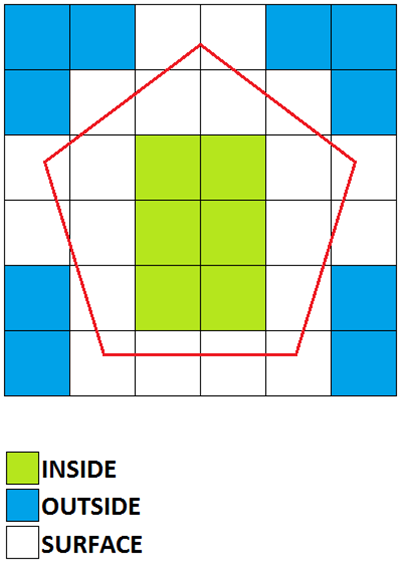
\includegraphics[width=0.4\textwidth]{classification}
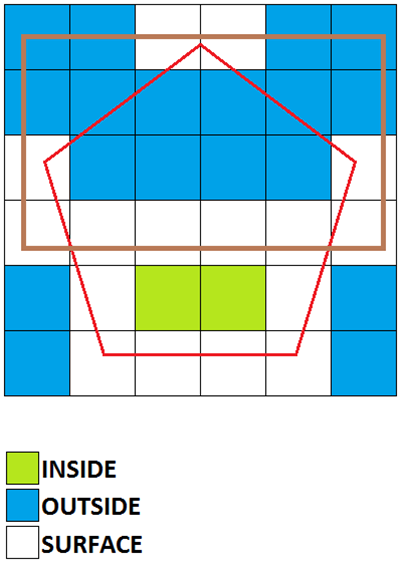
\includegraphics[width=0.4\textwidth]{classification_sub}
\caption{Principle of classifying cells of a grid according to the added mesh. Only surface cells are relevant for ray casting. The sketch on the left side shows the classified stock volume. On the right side the classification result, after a subtraction volume has been added, is shown.}
\label{fig:classification}
\end{figure}

When a new mesh is added to the grid, the mesh is again classified and merged into the existing cell classification. Limiting the modifiability of the scene by only allowing the addition of further subtraction volumes simplifies the rules for merging a new mesh into the grid as shown in Table \ref{tbl:classification_rules}.

\begin{table}[h]
\centering
\begin{tabular}{|c|c|c|c|c|}
\hline
\multicolumn{2}{|c|}{\multirow{2}{*}{merge}} & \multicolumn{3}{c|}{Cell class of subtraction volume} \\
\cline{3-5}
\multicolumn{2}{|c|}{} & outside & surface & inside \\
 \hline
\multirow{3}{*}{Cell class before} & outside & outside & outside & outside \\
\cline{2-5}
 & surface & surface & surface & outside \\
\cline{2-5}
 & inside & inside & surface & outside \\
\hline
\end{tabular}
\caption{Table of different merge scenarios and their outcome.}
\label{tbl:classification_rules}
\end{table}

Cells which are outside the added subtraction volume remain unchanged. Surface cells of the added volume become surface cells except they where outside cells before, and cells inside a subtraction volume always become outside cells, as they lie outside the resulting geometry. The result of merging a subtraction volume into the grid is visualized in the right sketch in Figure \ref{fig:classification}.

As we can see, cells which where surface cells before and contained triangles have now changed to outside cells and are therefore no longer relevant for ray casting. As a result, the increase of triangles in the surface cells by adding new volumes has been compensated by exclusion of some surface cells. This reduction of potential triangles for intersection with an increasing number of subtraction volumes is vital, as it enables scalability, allowing even scenes with thousands of subtraction volumes to be ray casted efficiently. In fact, some scenes can even be casted faster with an increasing number of subtraction volumes as the number of relevant surface cells and therefore triangles decreases.

However, this kind of reduction has a significant consequence on the ray casting algorithm. As subtraction volumes are divided into grid cells and some of them discarded, the volumes are no longer water-tight. This is a problem for entry/exit counting ray casting algorithms such as the one discussed in chapter \ref{sec:boolean_raycasting}. Therefore, an adapted version of this algorithm has to be developed, capable of handling open volumes. Chapter \ref{sec:adapted_ray_casting} discusses a method of getting around this problem.


\subsection{Improved counting algorithm}
\label{sec:adapted_ray_casting}

The entry and exit counting ray casting algorithm for boolean subtraction volumes discussed in Chapter \ref{sec:boolean_raycasting} maintains a counter value for each ray along the full traversal of the grid cells. However, by using the classification technique introduced in Chapter \ref{sec:classification} to eliminate irrelevant triangles, it is no longer possible to keep states between multiple cells, as some of them might not contain relevant triangles for intersection but might be important for state changes. For example, an entry into a subtraction volume inside an outside cell. Consequently, all required states of the ray can only and must be determined upon entry of a surface cell.

This problem mainly concerns the counter of each ray used to count the volume entries and exits along the ray in order to find the surface hit. To put it differently, each ray has to know inside how many subtraction volumes the ray is at the point where it enters a surface cell. However, if we have another look at the classified grid in Figure \ref{fig:classification}, we can see that each surface cell contains triangles from all subtraction volumes, called structures in code, inside which the ray can potentially be depending on its entry point. If the ray would be inside a subtraction volume which has no triangles inside the cell, the cell would have been classified as an inside cell of this volume and the cell would be skipped during ray casting.

Determining the number of subtraction volumes the entry point lies inside of, which is called inside counter, can be done by creating secondary rays. These rays are casted from the cell entry point of the initial ray, which is called primary ray for distinction, to a reference point on one triangle of each subtraction volume. The secondary ray must not hit other triangles of the same volume between the entry point and the triangle reference point. The used reference points on the triangles have to be inside the cell's bounding box and should not lie on a edge of the triangle, as numerical instability increases at the edges. A good candidate for such points is the centroid of the triangle clipped against the cell's bounding box. The angle between the secondary ray and the surface normal of the chosen triangle determines if the entry point is inside the volume the triangle belongs to. If the primary ray already hits a subtraction volume, no secondary ray is necessary for this volume and the primary rays direction and the surface normal of the hit triangle can be used instead. Figure \ref{fig:inside_counter} shows the determination of the inside counter on an example cell.

\begin{figure}
\centering
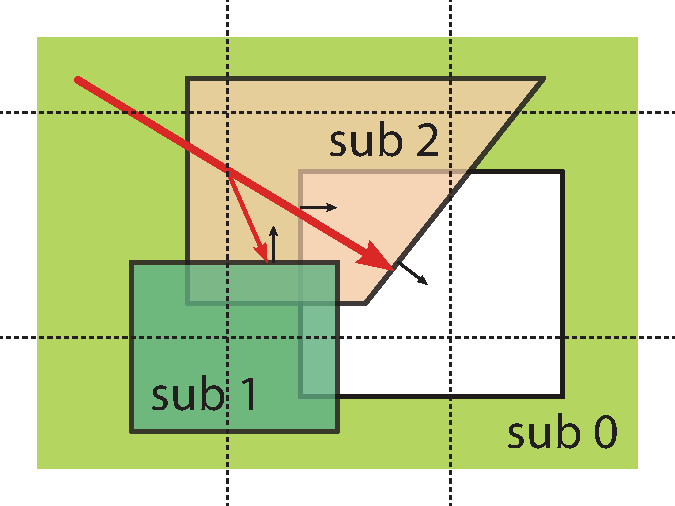
\includegraphics[width=0.5\textwidth]{inside_counter}
\caption{Determination of the inside counter upon cell entry. The primary ray hits the structures sub 0 and sub 2. Both surface normals enclose an angle with the ray's direction smaller than 90$^\circ$. Therefore, the ray's entry point lies inside of sub 0 and sub 2. As the primary ray does not hit sub 1, a secondary ray is sent to a reference point on a triangle of sub 1. As the surface normal and the ray's direction enclose an angle larger than 90$^\circ$, the cell entry point lies outside of sub 1. Therefore, the inside counter of the ray is initialized with minus two.}
\label{fig:inside_counter}
\end{figure}


\section{OpenCL ray caster}

\subsection{Data structure}

\subsection{Traversion}

\subsubsection{3DDA}

\subsubsection{Slice traverser}

\subsection{Implementations}

\subsection{Optimizations}

\subsection{Problems}



\section{Results}
\label{sec:results}


\subsection{Benchmarks and comparison with existing casters}



different scenes, casting times, visual appearance (missing pixels etc.)

\subsection{Development}

tools, debugger, VS integration

\subsection{Existing problems}

register consumption per work item (intersection buffer)

branch divergence

non coalesced memory access

\section{Summary and conclusion}
\label{sec:summary}

The RISC Software GmbH is a limited liability company and part of the software park Hagenberg. It focuses on the practical application of research done in the corresponding RISC institute. In mid 2011, the project Enlight was started with financial help by the governmental Regio 13 program. The goal of Enlight is to create a ray casting solution for interactive visualization of complex geometries consisting. Subtractive manufacturing is the main inspiration for the project. At the start of the internship in April 2013, most functionality was already implemented. The goal was therefore to try a different ray casting approach using GPGPU computing and OpenCL.

Ray casting is a wide spread technique for creating a two-dimensional image of a three-dimensional scene by casting rays from a camera position through the pixels of an image plane in space on which the final image should be projected. Ray casting has a different run time complexity than traditional rasterization, from which especially large scenes benefit. Ray casting also allows to easily generate images of implicit geometries like CSG models, where the scene is described by boolean combination of volumes. Counters are used in this case to count volume entries and exits until the surface hit is found. To accelerate ray casting several data structures are used to organize the scene more efficiently. One of them are regular grids, where the scene is subdivided into equally sized cubes. Grids are advantageous over other wide-spread data structures like kd trees for being easy and fast in construction, better facilitating dynamic scenes. During ray casting, grids are traversed by individual rays using a 3D variant of the DDA algorithm. Ray packets are guided through the grid slice by slice.

OpenCL is an open and free standard for parallel and general purpose programming targeting heterogeneous platforms. It is most often used to write programs, called kernels, for GPUs. To use OpenCL in an application, an SDK is required to provided the necessary header files and libraries. A typical OpenCL application starts by selecting an available platform and device as well as creating a context and a command queue. Kernels are written in OpenCL C and compiled at run time for the chosen device. Buffers may be created to pass larger blocks of data between the host application and a kernel. Kernels are executed in an n-dimensional range which determines the number of work items which should be executed. The memory model of OpenCL closely resembles modern GPUs by distinguishing between global, local, private (registers) and constant memory.

The existing prototype at the time the internship started is a C++ application built using Visual Studio and Intel's C++ compiler. It heavily uses AVX intrinsics to process ray packets as fast as possible in a SIMD fashion, thus limiting the application to newer processor types. The acceleration structure used is a regular grid. By classifying the grid cells every time a subtraction volume is added, the relevant cells for ray casting can be detected leading to a further reduction of intersection tests. By using subtraction volumes to express complex geometries, the ray casting algorithm has to use counters for volume entries and exists in order to find the implicit surface.

During the internship, several OpenCL ray casters have been developed together with a small OpenCL driver running these casters. Mainly single ray variants where focuses, as they involve no synchronization between individual rays. Several advanced features were added such as double precision support, source file embedding and out of core ray casting. The built infrastructure was finally ported to a new prototype which will be used for public demonstration and provides the base for a final product.

The benchmark results show that the OpenCL implementation can definitely compete with the existing CPU variant with a speedup of two to four on different scenes using single precision. The visual quality of the output is can be considered equal with the CPU double precision implementation. During development, several tools have been tried and evaluated. However, a few problems still remain which could further improve the ray casting performance on GPUs.

In conclusion it can be said that the OpenCL port of the ray caster was successful. Ray casting offers a lot of parallelism due to its parallel nature which can be advantageously used in GPGPU computing. However, we also saw that writing programs for the GPU as not as easy as developing an algorithm on the CPU. Commonly used and well-established concepts like dynamic allocation and communication methods between threads are suddenly unavailable when programming using OpenCL. Different aspects like memory access patterns, branch divergence between threads and register footprint come into play which are usually neglected in traditional software development.

Although the general purpose graphics processing unit becomes more and more capable of executing non-graphical tasks and running algorithms very dissimilar to the ones the a GPU was initially designed for, GPUs are still not general purpose processors. A graphic card remains a highly specialized instruments with its main goal of accelerating computer graphics. Therefore, only a small subset of problems actually benefits from being run on a GPU. Ray casting is fortunately one of them. Although we have also seen, that less independently parallel approaches, like the packet ray caster, which requires a high amount of synchronization, lead to a drastic loss of throughput.

Finally, also the developer tools available for OpenCL are far from being as satisfying as their CPU counterparts. During the internship, Intel's VTune Amplifier has been used for optimizing CPU code and was amazingly helpful. Also debugging C++ code, even if run in multiple threads, is well supported by today's debuggers (like the one integrated in Visual Studio). GPGPU computing is still a young discipline, also for vendors. The provided tools seem to be immature and unstable in several cases (e.g. Intel's OpenCL debugger or AMD's CodeXL). Some tools are also only available on a certain kind of hardware (e.g. NVIDIA's Visual Profiler or AMD's CodeXL). Although consequent improvements and advances are being made, there is still a lot of work to do to make GPU development (especially with OpenCL) as convenient and easy as traditional CPU orientated software development.

Concerning the future of Enlight, the initial planning schedules the project's end to December 2013. During this time, a lot of innovative work has been made which has been submitted to various conferences. Especially the idea of classification was new and proved to largely accelerate the ray casting of scenes described by subtractive volumes. RISC is currently discussing the integration of the ray casting technique developed during Enlight into other customer products, thus bringing the gained knowledge to its application. Furthermore, a follow-up project is in consideration, which may evaluate ray casting using a different but promising new piece of hardware on the high performance market, Intel's many integrated core (MIC) co processor cards. By being designed for massively parallel acceleration using existing software technologies and languages, Intel's MIC architecture does not suffer from the design requirements of a GPU, as it consists of a huge array of conventional Intel x86 cores. Who wants to be annoyed by GPGPU computing then?


\addcontentsline{toc}{section}{List of figures}
\renewcommand\listfigurename{List of figures}
\listoffigures

\clearpage

\addcontentsline{toc}{section}{List of listings}
\renewcommand\lstlistlistingname{List of listings} 
\lstlistoflistings

\clearpage

\addcontentsline{toc}{section}{References}
%\appto{\bibsetup}{\emergencystretch=1em}
\setcounter{biburllcpenalty}{9000}
\printbibliography[title=References]

\appendix
\section{Appendix}

\subsection{Matrix multiplication chart data}
\label{sec:matrix_mul_chart_data}

\subsubsection{Naive CPU}

\begin{tabular}{r r r}
size & run time mean & run time deviation \\
1 & 0 & 0 \\
25 & 0,000018 & 0 \\
50 & 0,000149 & 0,000019 \\
75 & 0,000524 & 0,000031 \\
100 & 0,001227 & 0,000156 \\
200 & 0,009001 & 0,000352 \\
300 & 0,035097 & 0,000099 \\
400 & 0,081693 & 0,000048 \\
500 & 0,198807 & 0,00369 \\
600 & 0,446807 & 0,022159 \\
700 & 0,885177 & 0,195293 \\
800 & 3,404683 & 0,063133 \\
900 & 6,094824 & 0,095358 \\
1000 & 9,158203 & 0,067449 \\
1100 & 12,273643 & 0,255862 \\
1200 & 16,473761 & 0,053628 \\
1300 & 20,301222 & 0,243348 \\
1400 & 25,209266 & 0,313975 \\
1500 & 30,550882 & 0,005375 \\
1600 & 39,762075 & 0,066254 \\
1700 & 44,930466 & 0,283708 \\
1800 & 54,965556 & 0,720861 \\
1900 & 61,130207 & 0,186277 \\
2000 & 74,531188 & 0,211783 \\
2100 & 83,185726 & 0,294925 \\
2200 & 96,555736 & 0,011703 \\
2300 & 110,60543 & 0,085392 \\
2400 & 133,480428 & 0,092403 \\
2500 & 142,234335 & 0,241012 \\
2600 & 161,313258 & 0,166381 \\
2700 & 181,084228 & 0,426846 \\
2800 & 210,357538 & 1,604625 \\
2900 & 229,775846 & 0,104415 \\
3000 & 263,874226 & 0,146529 \\
3100 & 286,894302 & 1,15429 \\
3200 & 314,497279 & 0,93643 \\
3300 & 345,02634 & 0,804373 \\
3400 & 397,331989 & 0,157337 \\
3500 & 436,245888 & 1,077226 \\
3600 & 488,217435 & 1,013651 \\
3700 & 525,113808 & 1,147087 \\
3800 & 560,915371 & 12,134538 \\
3900 & 624,880278 & 0,970673 \\
4000 & 657,499788 & 7,276395 \\
\end{tabular}

\subsubsection{OpenMP CPU}

\begin{tabular}{r r r}
size & run time mean & run time deviation \\
1 & 0,000201 & 0,000243 \\
25 & 0,000038 & 0,000001 \\
50 & 0,000124 & 0,000024 \\
75 & 0,000337 & 0,000039 \\
100 & 0,000679 & 0,000004 \\
200 & 0,006593 & 0,00036 \\
300 & 0,025074 & 0,000875 \\
400 & 0,065272 & 0,003128 \\
500 & 0,12838 & 0,002369 \\
600 & 0,464459 & 0,011541 \\
700 & 0,863346 & 0,0978 \\
800 & 1,776675 & 0,058818 \\
900 & 2,920025 & 0,047825 \\
1000 & 4,292602 & 0,02397 \\
1100 & 5,779423 & 0,032466 \\
1200 & 7,612406 & 0,08626 \\
1300 & 9,696026 & 0,027816 \\
1400 & 12,134429 & 0,055001 \\
1500 & 15,762018 & 0,196349 \\
1600 & 19,813159 & 0,294983 \\
1700 & 22,466314 & 0,229691 \\
1800 & 26,122541 & 0,089804 \\
1900 & 30,893081 & 0,208651 \\
2000 & 36,715405 & 0,271032 \\
2100 & 42,121322 & 0,025874 \\
2200 & 48,680537 & 0,143346 \\
2300 & 57,262861 & 0,705831 \\
2400 & 64,834907 & 0,097273 \\
2500 & 73,534766 & 0,18417 \\
2600 & 82,970566 & 0,135356 \\
2700 & 93,526126 & 0,38893 \\
2800 & 104,260969 & 0,467199 \\
2900 & 117,205018 & 0,35524 \\
3000 & 130,497517 & 0,991553 \\
3100 & 144,324302 & 1,200542 \\
3200 & 168,570176 & 1,039508 \\
3300 & 175,129977 & 0,230182 \\
3400 & 195,68473 & 1,115665 \\
3500 & 214,542733 & 0,94702 \\
3600 & 236,730639 & 0,425485 \\
3700 & 258,485694 & 0,532694 \\
3800 & 277,081415 & 1,662909 \\
3900 & 302,396295 & 0,657581 \\
4000 & 323,586431 & 2,265068 \\
\end{tabular}

\subsubsection{CBLAS CPU}

\begin{tabular}{r r r}
size & run time mean & run time deviation \\
1 & 0,000005 & 0,000007 \\
25 & 0,00001 & 0 \\
50 & 0,000059 & 0 \\
75 & 0,000192 & 0,000001 \\
100 & 0,00039 & 0,000003 \\
200 & 0,003063 & 0,000137 \\
300 & 0,012551 & 0,000072 \\
400 & 0,029367 & 0,000024 \\
500 & 0,056781 & 0,000061 \\
600 & 0,099672 & 0,001023 \\
700 & 0,201223 & 0,051646 \\
800 & 0,333364 & 0,086883 \\
900 & 0,456633 & 0,025736 \\
1000 & 0,678157 & 0,026632 \\
1100 & 0,887394 & 0,017413 \\
1200 & 1,219493 & 0,05202 \\
1300 & 1,494735 & 0,022683 \\
1400 & 1,896388 & 0,04717 \\
1500 & 2,315734 & 0,037512 \\
1600 & 2,858037 & 0,031083 \\
1700 & 3,508918 & 0,094538 \\
1800 & 4,086062 & 0,051909 \\
1900 & 4,806106 & 0,097737 \\
2000 & 5,62859 & 0,066646 \\
2100 & 6,078531 & 0,005372 \\
2200 & 6,998793 & 0,008354 \\
2300 & 8,031067 & 0,034976 \\
2400 & 9,107732 & 0,014117 \\
2500 & 10,299053 & 0,021374 \\
2600 & 11,575173 & 0,004663 \\
2700 & 12,983403 & 0,07307 \\
2800 & 14,490919 & 0,084496 \\
2900 & 16,092239 & 0,040324 \\
3000 & 17,804858 & 0,024317 \\
3100 & 19,637134 & 0,017677 \\
3200 & 21,580045 & 0,037946 \\
3300 & 23,737392 & 0,07079 \\
3400 & 25,977898 & 0,012364 \\
3500 & 28,343538 & 0,042341 \\
3600 & 31,180217 & 0,113045 \\
3700 & 33,803832 & 0,033084 \\
3800 & 37,478187 & 0,154286 \\
3900 & 39,98611 & 0,102763 \\
4000 & 43,48911 & 0,097813 \\
\end{tabular}

\subsubsection{Naive GPU}

\begin{tabular}{r r r r r r r r r}
size & upload time mean  & upload time deviation & run time mean & run time deviation & download time mean & download time deviation & wg size & up run down sum \\
1 & 0,00088 & 0,000671 & 0,000615 & 0,000291 & 0,000515 & 0,000098 & 16 & 0,002011 \\
25 & 0,002313 & 0,001245 & 0,001516 & 0,000214 & 0,001091 & 0,000138 & 16 & 0,00492 \\
50 & 0,000605 & 0,000246 & 0,000515 & 0,000122 & 0,000537 & 0,000069 & 16 & 0,001656 \\
75 & 0,001388 & 0,001341 & 0,000616 & 0,000189 & 0,000544 & 0,00006 & 16 & 0,002547 \\
100 & 0,000791 & 0,000289 & 0,000668 & 0,000095 & 0,000509 & 0,000021 & 16 & 0,001967 \\
200 & 0,000966 & 0,000187 & 0,002478 & 0,000078 & 0,000755 & 0,000027 & 16 & 0,0042 \\
300 & 0,00111 & 0,000203 & 0,006948 & 0,000004 & 0,00081 & 0,000043 & 16 & 0,008867 \\
400 & 0,001459 & 0,000156 & 0,015373 & 0,00003 & 0,000997 & 0,000004 & 16 & 0,017829 \\
500 & 0,001692 & 0,000255 & 0,0295 & 0,000057 & 0,001021 & 0,000054 & 16 & 0,032213 \\
600 & 0,002086 & 0,000095 & 0,049811 & 0,000103 & 0,001417 & 0,000168 & 16 & 0,053314 \\
700 & 0,002627 & 0,000152 & 0,078352 & 0,000156 & 0,001593 & 0,000111 & 16 & 0,082571 \\
800 & 0,003309 & 0,000287 & 0,116651 & 0,00038 & 0,002011 & 0,000312 & 16 & 0,121971 \\
900 & 0,003735 & 0,000176 & 0,166536 & 0,000032 & 0,002247 & 0,00034 & 16 & 0,172518 \\
1000 & 0,004558 & 0,000344 & 0,226959 & 0,000215 & 0,002512 & 0,000296 & 16 & 0,234028 \\
1100 & 0,005154 & 0,000159 & 0,300857 & 0,000079 & 0,00294 & 0,000401 & 16 & 0,308951 \\
1200 & 0,006172 & 0,000451 & 0,390213 & 0,000503 & 0,003762 & 0,00116 & 16 & 0,400147 \\
1300 & 0,007018 & 0,000246 & 0,498331 & 0,00018 & 0,003791 & 0,000678 & 16 & 0,50914 \\
1400 & 0,007851 & 0,000166 & 0,619719 & 0,000168 & 0,004264 & 0,000638 & 16 & 0,631833 \\
1500 & 0,00894 & 0,000164 & 0,760697 & 0,000259 & 0,004787 & 0,000716 & 16 & 0,774423 \\
1600 & 0,010071 & 0,000208 & 0,922575 & 0,000214 & 0,00528 & 0,000799 & 16 & 0,937926 \\
1700 & 0,011411 & 0,000169 & 1,110858 & 0,000437 & 0,00588 & 0,000912 & 16 & 1,128149 \\
1800 & 0,012665 & 0,000253 & 1,314582 & 0,000277 & 0,006421 & 0,001081 & 16 & 1,333667 \\
1900 & 0,013955 & 0,00022 & 1,543945 & 0,000435 & 0,007093 & 0,001145 & 16 & 1,564993 \\
2000 & 0,015383 & 0,00025 & 1,800036 & 0,000517 & 0,007745 & 0,001241 & 16 & 1,823163 \\
2100 & 0,018453 & 0,001132 & 2,089494 & 0,000709 & 0,00891 & 0,001781 & 16 & 2,116857 \\
2200 & 0,020629 & 0,001056 & 2,396777 & 0,00101 & 0,009662 & 0,001862 & 16 & 2,427068 \\
2300 & 0,021557 & 0,001121 & 2,73565 & 0,000838 & 0,010521 & 0,002003 & 16 & 2,767727 \\
2400 & 0,023792 & 0,001303 & 3,108474 & 0,00053 & 0,012114 & 0,002304 & 16 & 3,14438 \\
2500 & 0,025764 & 0,000829 & 3,525107 & 0,001671 & 0,013198 & 0,003711 & 16 & 3,564069 \\
2600 & 0,030394 & 0,003931 & 3,95678 & 0,000505 & 0,013523 & 0,002903 & 16 & 4,000697 \\
2700 & 0,02907 & 0,001087 & 4,425657 & 0,000171 & 0,014466 & 0,003151 & 16 & 4,469194 \\
2800 & 0,031051 & 0,001214 & 4,935096 & 0,000193 & 0,015604 & 0,00332 & 16 & 4,981752 \\
2900 & 0,034663 & 0,000787 & 5,499003 & 0,000063 & 0,018825 & 0,002719 & 16 & 5,55249 \\
3000 & 0,03674 & 0,000772 & 6,076687 & 0,000326 & 0,019522 & 0,002762 & 16 & 6,132948 \\
3100 & 0,039193 & 0,000626 & 6,699122 & 0,000248 & 0,020904 & 0,002895 & 16 & 6,759219 \\
3200 & 0,042414 & 0,000287 & 7,366433 & 0,000382 & 0,02241 & 0,003427 & 16 & 7,431257 \\
3300 & 0,044612 & 0,000872 & 8,098219 & 0,000295 & 0,023677 & 0,003526 & 16 & 8,166509 \\
3400 & 0,047597 & 0,000858 & 8,845134 & 0,001031 & 0,02558 & 0,003803 & 16 & 8,918311 \\
3500 & 0,05071 & 0,000831 & 9,642507 & 0,000035 & 0,026813 & 0,00355 & 16 & 9,720029 \\
3600 & 0,054842 & 0,000794 & 10,488255 & 0,000327 & 0,028352 & 0,003967 & 16 & 10,571449 \\
3700 & 0,05736 & 0,001358 & 11,412625 & 0,000414 & 0,031272 & 0,00441 & 16 & 11,501257 \\
3800 & 0,06071 & 0,001305 & 12,344899 & 0,000137 & 0,031608 & 0,004524 & 16 & 12,437216 \\
3900 & 0,064896 & 0,001158 & 13,335906 & 0,000247 & 0,033453 & 0,004929 & 16 & 13,434255 \\
4000 & 0,068064 & 0,001656 & 14,3872 & 0,000152 & 0,035069 & 0,00478 & 16 & 14,490333 \\
\end{tabular}

\subsubsection{Tiles GPU}

\begin{tabular}{r r r r r r r r r}
size & upload time mean  & upload time deviation & run time mean & run time deviation & download time mean & download time deviation & wg size & up run down sum \\
1 & 0,002448 & 0,001914 & 0,000439 & 0,0003 & 0,000479 & 0,000025 & 16 & 0,003365 \\
25 & 0,001442 & 0,000625 & 0,000323 & 0,000064 & 0,000495 & 0,000073 & 16 & 0,00226 \\
50 & 0,00142 & 0,000421 & 0,00036 & 0,000063 & 0,000495 & 0,000036 & 16 & 0,002275 \\
75 & 0,00147 & 0,000174 & 0,000391 & 0,000076 & 0,000528 & 0,00005 & 16 & 0,002389 \\
100 & 0,002443 & 0,001676 & 0,000485 & 0,000116 & 0,00057 & 0,000092 & 16 & 0,003498 \\
200 & 0,001545 & 0,000168 & 0,001096 & 0,000081 & 0,000638 & 0,000008 & 16 & 0,003278 \\
300 & 0,001548 & 0,000208 & 0,002783 & 0,000163 & 0,00069 & 0,000017 & 16 & 0,005022 \\
400 & 0,001627 & 0,000374 & 0,006297 & 0,000704 & 0,0007 & 0,000027 & 16 & 0,008624 \\
500 & 0,004134 & 0,000871 & 0,012672 & 0,000636 & 0,001544 & 0,000655 & 16 & 0,01835 \\
600 & 0,004918 & 0,003085 & 0,02007 & 0,000656 & 0,001241 & 0,000179 & 16 & 0,026228 \\
700 & 0,004176 & 0,000242 & 0,03017 & 0,000284 & 0,001945 & 0,000232 & 16 & 0,036292 \\
800 & 0,003685 & 0,000578 & 0,043927 & 0,000173 & 0,001753 & 0,000092 & 16 & 0,049366 \\
900 & 0,005105 & 0,000381 & 0,064656 & 0,000157 & 0,00251 & 0,000281 & 16 & 0,07227 \\
1000 & 0,006008 & 0,000638 & 0,087169 & 0,00019 & 0,002756 & 0,000313 & 16 & 0,095933 \\
1100 & 0,006902 & 0,000576 & 0,114304 & 0,000105 & 0,003318 & 0,000413 & 16 & 0,124525 \\
1200 & 0,006605 & 0,000468 & 0,146479 & 0,000256 & 0,003784 & 0,001259 & 16 & 0,156868 \\
1300 & 0,009367 & 0,00067 & 0,191224 & 0,000231 & 0,004236 & 0,000574 & 16 & 0,204827 \\
1400 & 0,010644 & 0,000606 & 0,236014 & 0,000353 & 0,004866 & 0,000603 & 16 & 0,251525 \\
1500 & 0,012009 & 0,000589 & 0,287541 & 0,000299 & 0,00545 & 0,00069 & 16 & 0,304999 \\
1600 & 0,011138 & 0,000652 & 0,346084 & 0,00037 & 0,005234 & 0,00081 & 16 & 0,362457 \\
1700 & 0,015061 & 0,000866 & 0,423549 & 0,000395 & 0,006813 & 0,000875 & 16 & 0,445422 \\
1800 & 0,016781 & 0,000887 & 0,498664 & 0,000468 & 0,007173 & 0,0011 & 16 & 0,522618 \\
1900 & 0,019054 & 0,000745 & 0,581821 & 0,0008 & 0,007855 & 0,001123 & 16 & 0,608729 \\
2000 & 0,017004 & 0,00086 & 0,67445 & 0,000655 & 0,007657 & 0,001288 & 16 & 0,699111 \\
2100 & 0,022306 & 0,001388 & 0,793803 & 0,000599 & 0,010148 & 0,001706 & 16 & 0,826257 \\
2200 & 0,024483 & 0,001279 & 0,906879 & 0,000653 & 0,010497 & 0,001939 & 16 & 0,94186 \\
2300 & 0,026937 & 0,001193 & 1,030812 & 0,000751 & 0,011485 & 0,002201 & 16 & 1,069233 \\
2400 & 0,023442 & 0,001087 & 1,165678 & 0,000061 & 0,011712 & 0,002528 & 16 & 1,200832 \\
2500 & 0,031477 & 0,001602 & 1,335873 & 0,000281 & 0,013502 & 0,002752 & 16 & 1,380852 \\
2600 & 0,034149 & 0,001601 & 1,494898 & 0,000155 & 0,015364 & 0,003125 & 16 & 1,544412 \\
2700 & 0,03642 & 0,001945 & 1,665676 & 0,000042 & 0,016242 & 0,003312 & 16 & 1,718339 \\
2800 & 0,031189 & 0,001232 & 1,849724 & 0,000336 & 0,015738 & 0,003504 & 16 & 1,896652 \\
2900 & 0,04386 & 0,001234 & 2,079821 & 0,000051 & 0,019342 & 0,002732 & 16 & 2,143023 \\
3000 & 0,046835 & 0,00126 & 2,292093 & 0,000189 & 0,020772 & 0,002852 & 16 & 2,3597 \\
3100 & 0,049822 & 0,001252 & 2,518337 & 0,000238 & 0,021931 & 0,003008 & 16 & 2,590089 \\
3200 & 0,04179 & 0,000877 & 2,761665 & 0,000378 & 0,022967 & 0,003495 & 16 & 2,826421 \\
3300 & 0,058773 & 0,002924 & 3,059096 & 0,000131 & 0,024915 & 0,003402 & 16 & 3,142784 \\
3400 & 0,060329 & 0,0016 & 3,333357 & 0,000107 & 0,026094 & 0,003542 & 16 & 3,419781 \\
3500 & 0,06534 & 0,0029 & 3,621535 & 0,000386 & 0,027677 & 0,003944 & 16 & 3,714553 \\
3600 & 0,054482 & 0,001003 & 3,927815 & 0,000615 & 0,028413 & 0,004473 & 16 & 4,01071 \\
3700 & 0,073444 & 0,001872 & 4,307183 & 0,000406 & 0,030629 & 0,00444 & 16 & 4,411256 \\
3800 & 0,076639 & 0,001961 & 4,648022 & 0,000217 & 0,03249 & 0,004736 & 16 & 4,757151 \\
3900 & 0,081102 & 0,002062 & 5,006632 & 0,000382 & 0,034148 & 0,00499 & 16 & 5,121882 \\
4000 & 0,07853 & 0,014639 & 5,385155 & 0,000519 & 0,041405 & 0,007665 & 16 & 5,50509 \\
\end{tabular}

\subsubsection{Blocks GPU}

\begin{tabular}{r r r r r r r r r}
size & upload time mean  & upload time deviation & run time mean & run time deviation & download time mean & download time deviation & wg size & up run down sum \\
1 & 0,004364 & 0,000277 & 0,001491 & 0,000528 & 0,001355 & 0,000095 & 16 & 0,007211 \\
25 & 0,003867 & 0,001188 & 0,00127 & 0,000035 & 0,000983 & 0,000061 & 16 & 0,00612 \\
50 & 0,003267 & 0,000632 & 0,001104 & 0,000112 & 0,000957 & 0,000024 & 16 & 0,005328 \\
75 & 0,003893 & 0,000826 & 0,001284 & 0,000133 & 0,000956 & 0,000012 & 16 & 0,006133 \\
100 & 0,001828 & 0,000122 & 0,001004 & 0,000116 & 0,000521 & 0,000043 & 16 & 0,003353 \\
200 & 0,000899 & 0,000219 & 0,000675 & 0,000193 & 0,0004 & 0,000014 & 16 & 0,001974 \\
300 & 0,001062 & 0,000202 & 0,000923 & 0,000091 & 0,000476 & 0,000013 & 16 & 0,002461 \\
400 & 0,001477 & 0,000234 & 0,00148 & 0,000116 & 0,00055 & 0,000014 & 16 & 0,003507 \\
500 & 0,001627 & 0,00027 & 0,002842 & 0,000124 & 0,000707 & 0,000012 & 16 & 0,005175 \\
600 & 0,003553 & 0,000117 & 0,004975 & 0,00013 & 0,00128 & 0,000032 & 16 & 0,009809 \\
700 & 0,004376 & 0,000071 & 0,007908 & 0,000177 & 0,001557 & 0,000024 & 16 & 0,013841 \\
800 & 0,005056 & 0,000264 & 0,009433 & 0,000265 & 0,001807 & 0,000032 & 16 & 0,016296 \\
900 & 0,00603 & 0,000171 & 0,016618 & 0,000202 & 0,00239 & 0,000164 & 16 & 0,025038 \\
1000 & 0,005701 & 0,000338 & 0,019658 & 0,00014 & 0,002507 & 0,000088 & 16 & 0,027865 \\
1100 & 0,006451 & 0,000359 & 0,027679 & 0,000162 & 0,002923 & 0,000196 & 16 & 0,037053 \\
1200 & 0,007434 & 0,000387 & 0,02952 & 0,000214 & 0,00357 & 0,00074 & 16 & 0,040524 \\
1300 & 0,00856 & 0,000069 & 0,045869 & 0,000249 & 0,003928 & 0,000495 & 16 & 0,058358 \\
1400 & 0,009766 & 0,000247 & 0,05146 & 0,000545 & 0,005348 & 0,000734 & 16 & 0,066573 \\
1500 & 0,010896 & 0,00014 & 0,068606 & 0,000279 & 0,004966 & 0,000781 & 16 & 0,084468 \\
1600 & 0,01182 & 0,000311 & 0,068271 & 0,000658 & 0,0054 & 0,000767 & 16 & 0,08549 \\
1700 & 0,013058 & 0,000391 & 0,098584 & 0,000501 & 0,005967 & 0,000851 & 16 & 0,117608 \\
1800 & 0,014906 & 0,000794 & 0,118917 & 0,00097 & 0,006613 & 0,001 & 16 & 0,140436 \\
1900 & 0,015987 & 0,000491 & 0,135782 & 0,000562 & 0,007223 & 0,00108 & 16 & 0,158992 \\
2000 & 0,017662 & 0,000851 & 0,14032 & 0,000448 & 0,00789 & 0,001228 & 16 & 0,165872 \\
2100 & 0,018932 & 0,000748 & 0,185613 & 0,00075 & 0,008788 & 0,00182 & 16 & 0,213332 \\
2200 & 0,020697 & 0,000762 & 0,19472 & 0,000954 & 0,010356 & 0,00169 & 16 & 0,225774 \\
2300 & 0,022349 & 0,000806 & 0,263516 & 0,000653 & 0,010435 & 0,002105 & 16 & 0,2963 \\
2400 & 0,024078 & 0,000907 & 0,238453 & 0,000592 & 0,011544 & 0,002631 & 16 & 0,274075 \\
2500 & 0,026025 & 0,000837 & 0,316213 & 0,000317 & 0,012346 & 0,002533 & 16 & 0,354584 \\
2600 & 0,02789 & 0,00113 & 0,329413 & 0,000523 & 0,014654 & 0,002358 & 16 & 0,371957 \\
2700 & 0,029889 & 0,000981 & 0,397656 & 0,000093 & 0,014294 & 0,002866 & 16 & 0,441839 \\
2800 & 0,031888 & 0,000783 & 0,396998 & 0,001337 & 0,016416 & 0,003237 & 16 & 0,445302 \\
2900 & 0,035022 & 0,000289 & 0,491999 & 0,000149 & 0,018796 & 0,00263 & 16 & 0,545818 \\
3000 & 0,037224 & 0,000305 & 0,499876 & 0,000807 & 0,019717 & 0,002844 & 16 & 0,556817 \\
3100 & 0,039727 & 0,000418 & 0,607555 & 0,000786 & 0,021075 & 0,003069 & 16 & 0,668357 \\
3200 & 0,042457 & 0,000543 & 0,585249 & 0,003607 & 0,022503 & 0,003357 & 16 & 0,650209 \\
3300 & 0,045373 & 0,000665 & 0,727172 & 0,00024 & 0,023469 & 0,003611 & 16 & 0,796014 \\
3400 & 0,048175 & 0,000748 & 0,748447 & 0,000549 & 0,025088 & 0,003807 & 16 & 0,82171 \\
3500 & 0,051074 & 0,000705 & 0,845195 & 0,000689 & 0,026504 & 0,003892 & 16 & 0,922773 \\
3600 & 0,055183 & 0,001103 & 0,849574 & 0,000431 & 0,028227 & 0,004282 & 16 & 0,932984 \\
3700 & 0,05801 & 0,000982 & 1,011169 & 0,000397 & 0,030064 & 0,004658 & 16 & 1,099242 \\
3800 & 0,061369 & 0,001165 & 1,005228 & 0,000554 & 0,031837 & 0,004947 & 16 & 1,098435 \\
3900 & 0,065239 & 0,001164 & 1,177487 & 0,000593 & 0,033592 & 0,005467 & 16 & 1,276318 \\
4000 & 0,068455 & 0,001326 & 1,108897 & 0,000935 & 0,035007 & 0,006206 & 16 & 1,212359 \\
\end{tabular}

\subsubsection{Blocks and tiles GPU}

\begin{tabular}{r r r r r r r r r}
size & upload time mean  & upload time deviation & run time mean & run time deviation & download time mean & download time deviation & wg size & up run down sum \\
1 & 0,00254 & 0,002182 & 0,000422 & 0,000221 & 0,00051 & 0,000015 & 16 & 0,003473 \\
25 & 0,001337 & 0,000083 & 0,000347 & 0,000034 & 0,000729 & 0,000038 & 16 & 0,002413 \\
50 & 0,001564 & 0,000064 & 0,000373 & 0,000034 & 0,000752 & 0,000006 & 16 & 0,002688 \\
75 & 0,001597 & 0,000121 & 0,000423 & 0,000128 & 0,000627 & 0,000137 & 16 & 0,002647 \\
100 & 0,00166 & 0,000267 & 0,001106 & 0,001045 & 0,000804 & 0,000062 & 16 & 0,00357 \\
200 & 0,001892 & 0,000146 & 0,001145 & 0,000141 & 0,000962 & 0,000108 & 16 & 0,003999 \\
300 & 0,002126 & 0,000158 & 0,001408 & 0,000038 & 0,001596 & 0,000715 & 16 & 0,00513 \\
400 & 0,002434 & 0,000137 & 0,003426 & 0,00068 & 0,001237 & 0,000016 & 16 & 0,007098 \\
500 & 0,00407 & 0,001983 & 0,004605 & 0,000187 & 0,001242 & 0,000044 & 16 & 0,009918 \\
600 & 0,003373 & 0,000404 & 0,008245 & 0,000314 & 0,001707 & 0,00024 & 16 & 0,013326 \\
700 & 0,003855 & 0,000456 & 0,010752 & 0,000263 & 0,00186 & 0,000271 & 16 & 0,016467 \\
800 & 0,004272 & 0,000397 & 0,016709 & 0,000117 & 0,001973 & 0,000366 & 16 & 0,022954 \\
900 & 0,005308 & 0,000741 & 0,025691 & 0,000207 & 0,002415 & 0,000342 & 16 & 0,033414 \\
1000 & 0,006016 & 0,000511 & 0,034457 & 0,000141 & 0,002708 & 0,00041 & 16 & 0,043181 \\
1100 & 0,007276 & 0,000862 & 0,044562 & 0,000332 & 0,003282 & 0,000532 & 16 & 0,05512 \\
1200 & 0,008067 & 0,000605 & 0,05206 & 0,000176 & 0,00401 & 0,001056 & 16 & 0,064136 \\
1300 & 0,010145 & 0,000357 & 0,070472 & 0,00046 & 0,004582 & 0,000529 & 16 & 0,085199 \\
1400 & 0,010606 & 0,000658 & 0,080893 & 0,000226 & 0,004675 & 0,000728 & 16 & 0,096173 \\
1500 & 0,012143 & 0,000712 & 0,11148 & 0,000621 & 0,005316 & 0,000867 & 16 & 0,128939 \\
1600 & 0,012156 & 0,000449 & 0,117121 & 0,000255 & 0,005879 & 0,000627 & 16 & 0,135156 \\
1700 & 0,018285 & 0,000099 & 0,147038 & 0,000408 & 0,007887 & 0,000739 & 16 & 0,17321 \\
1800 & 0,020032 & 0,000216 & 0,182826 & 0,000644 & 0,008508 & 0,000824 & 16 & 0,211366 \\
1900 & 0,021572 & 0,000305 & 0,202793 & 0,000478 & 0,009292 & 0,001101 & 16 & 0,233657 \\
2000 & 0,023732 & 0,000361 & 0,293721 & 0,000172 & 0,010286 & 0,000902 & 16 & 0,327739 \\
2100 & 0,025338 & 0,000507 & 0,267278 & 0,000888 & 0,010508 & 0,001331 & 16 & 0,303124 \\
2200 & 0,02738 & 0,00079 & 0,318493 & 0,000652 & 0,011427 & 0,001414 & 16 & 0,357301 \\
2300 & 0,029166 & 0,000782 & 0,36735 & 0,000947 & 0,012938 & 0,001473 & 16 & 0,409454 \\
2400 & 0,031566 & 0,001266 & 0,411388 & 0,001157 & 0,013725 & 0,001873 & 16 & 0,45668 \\
2500 & 0,034303 & 0,001229 & 0,504502 & 0,000309 & 0,014413 & 0,002126 & 16 & 0,553218 \\
2600 & 0,036474 & 0,001953 & 0,512085 & 0,000335 & 0,015425 & 0,002384 & 16 & 0,563984 \\
2700 & 0,038968 & 0,001726 & 0,590179 & 0,000108 & 0,01625 & 0,002581 & 16 & 0,645397 \\
2800 & 0,041076 & 0,001856 & 0,664322 & 0,000836 & 0,017386 & 0,002915 & 16 & 0,722784 \\
2900 & 0,04695 & 0,00065 & 0,726595 & 0,000198 & 0,019761 & 0,002516 & 16 & 0,793306 \\
3000 & 0,049998 & 0,001159 & 0,770267 & 0,000264 & 0,022176 & 0,002482 & 16 & 0,842441 \\
3100 & 0,052778 & 0,000789 & 0,873651 & 0,000207 & 0,022381 & 0,002717 & 16 & 0,94881 \\
3200 & 0,045516 & 0,000144 & 0,92974 & 0,001365 & 0,02325 & 0,003414 & 16 & 0,998505 \\
3300 & 0,058981 & 0,001037 & 1,093571 & 0,000555 & 0,025335 & 0,003434 & 16 & 1,177887 \\
3400 & 0,062638 & 0,001015 & 1,172562 & 0,000231 & 0,026959 & 0,003084 & 16 & 1,262158 \\
3500 & 0,065681 & 0,001164 & 1,231127 & 0,000552 & 0,028065 & 0,003714 & 16 & 1,324872 \\
3600 & 0,071656 & 0,001267 & 1,37143 & 0,000861 & 0,029765 & 0,003979 & 16 & 1,472851 \\
3700 & 0,075867 & 0,001194 & 1,453368 & 0,002109 & 0,031364 & 0,004476 & 16 & 1,560598 \\
3800 & 0,079499 & 0,001346 & 1,681469 & 0,000753 & 0,032934 & 0,004797 & 16 & 1,793902 \\
3900 & 0,083834 & 0,001488 & 1,678507 & 0,000891 & 0,03473 & 0,005096 & 16 & 1,797071 \\
4000 & 0,087218 & 0,001696 & 1,845283 & 0,001991 & 0,036915 & 0,006114 & 16 & 1,969416 \\
\end{tabular}

\end{document}